\section{Auswertung}
\label{sec:Auswertung}

\subsection{Zählrohr-Charakteristik}
\label{subsec:Zählrohr-Charakteristik}
Die Charakteristik des Zählrohres wird anhand der Messergebnisse in die Abbildung \ref{fig:Charakteristik} aufgenommen.
Der Plateau-Bereich wird von 390 bis 610 $\si{\volt}$ angenommen, somit ist der Bereich 280 $\si{\volt}$ lang.
Mithilfe von ipython wird eine lineare Ausgleichsrechnung für den Plateau-Bereich durchgeführt, für die Ausgleichgerade ergibt sich:
\begin{equation*}
  N = (1.169 \pm 0.325)U + (9575.69 \pm 163.72)
\end{equation*}
Die Plateau-Steigung kann auch mit 101,22\% pro $\SI{100}{\volt}$ angegeben werden.
Eine geeignete Zählrohrspannung ist $\SI{400}{\volt}$, da diese etwas über der Spannung $U_\text{E}$ und im Auslösebereich liegt.
\begin{figure}
  \centering
  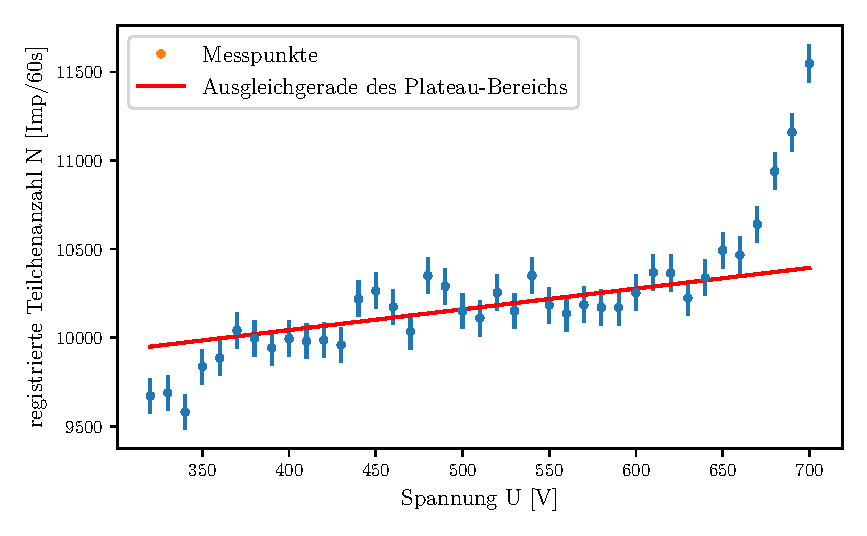
\includegraphics{Plateau_Gerade.pdf}
  \caption{Zählrohrcharakteristik mit Ausgleichgerade für den Plateau-Bereich.}
  \label{fig:Charakteristik}
\end{figure}

\subsection{Zeitlicher Abstand zwischen Primär- und Nachentladungsimpuls}
\label{subsec:Primär_Nachentladung}

\subsection{Bestimmung der Totzeit}
\label{subsec:Totzeit}

\subsubsection{Oszilloskop}
Anhand einer Momentaufnahme der Anzeige des Oszilloskops soll die Totzeit bestimmt werden.
Die Zeit zwischen dem ersten und zweitem Puls wird abgelesen und auf $\SI{100}{\mu\second}$ geschätzt.

\subsubsection{Zwei-Quellen-Methode}
Mit der Formel ... wird die Totzeit mit den folgenden Zählraten ermittelt:
\begin{align*}
  N_1 &= \frac{96041}{120} \text{Imp/s}
  N_{1+2} &= \frac{158479}{120} \text{Imp/s}
  N_2 &= \frac{76518}{120} \text{Imp/s}
\end{align*}
Mit der Fehlerfortpflanzung nach Gauß folgt insgesamt für die Totzeit $T = \SI{115 \pm 0.047}{\micro\second}$.